\section{Линейное пространство комплексных чисел}
\subsection{Основные определения}
\deff{Множество комплексных чисел} - линейное пространство \(\mathbb{R}^2\) с евклидовой нормой.(мы его так вводим).
Получаем первый вариант записи комплексных чисел - Декартову форму записи: $$(x; y)=z\in\mathbb{C}; x, y\in\mathbb{R}$$
Евклидову норму \(|z|=||(x;y)||_2=\sqrt{x^2 + y^2}\) называют модулем комплексного числа.

Представив комплексные числа таким образом, мы видим их геометрическую интерпретацию, как радиус-векторов на плоскости (модуль числа - длина радиус-вектора). В качестве базиса будем использовать вектора \((1;0)\) - вещественную единицу и \((0;1)\) - мнимую единицу, обозначаемую $i$.

\deff{Алгебраическая форма записи} - ещё один вариант записи комплексных чисел:
$$z=(x;y)=x+iy$$
При этом \(x=Re\,z\) - вещественная часть числа, а \(y=Im\,z\)ч - мнимая часть.

При \(x=0\) число становится чисто мнимым.

При \(y=0\) число можно отождествлять с вещественным числом \(x\).

Теперь можем ввести полярную систему координат с центром, совпадающим с центром декартовой системы координат и осью вдоль оси \(Re\,z\). Тогда для каждого ненулевого комплексного числа получим \(r\) и\(\varphi\). Для \(z=x+iy\neq0\) модуль числа \(r=\sqrt{x^2 + y^2}\), а \(\varphi\) - аргумент - такой угол, что \(\tan{\varphi}= x/y\) (Функция аргумента имеет своё обозначение \(\varphi=Arg(x+iy)\) или \(\varphi=\arg_k(x+iy)\), если хотим аргумент, как многозначную функцию и \(\varphi=\arg(x+iy)\) или \(\varphi=\arg_0(x+iy)\), если хотим получить главный аргумент, то есть значение аргумента лежащее в \([-\pi;\pi)\) или в \([0;2\pi)\) в зависимости от выбранного диапазона).
\begin{center}
    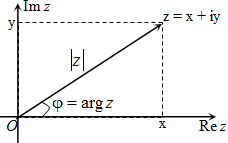
\includegraphics[width=5cm]{Images/Chapter_2/2-2-1.png}
\end{center}
Заметим, что тогда \(x=r\cos{\varphi}\), а \(y=r\sin{\varphi}\). Тогда получим третий вариант записи комплексного числа - Тригонометрическую форму записи: $$z=x+iy=r(\cos{\varphi}+i\sin{\varphi})$$
\subsection{Комплексные = алгебра с нормой.}

То, что это линейное пространство и так понятно (очевидно, что все 8 аксиом выполнены, тк мы до этого доказывали, что \(R^2\) --- линейное пространство). Давайте докажем, что комплексные - это \deff{нормированная алгебра}.

Значит, мы хотим создать такую операцию умножения, что она будет согласованно с нормой. Посмотрим, тогда чему должно быть равно \(i\cdot i = i^2\).

Тогда давайте предположим, что сейчас \(i\cdot i = \lambda + \phi i\).

Посмотрим, чему у нас будет равна вот такая норма:

$$ ||i^2+ix|| = ||i(i+x) || \leq ||i|| ||i+x|| = \sqrt{1+x^2}$$

Должно выполняться последнее, если мы хотим, чтобы норма была согласованна с умножением. Но мы знаем что  \(i\cdot i = \lambda + \phi i\)! Подставим:

$$||i^2+ix|| = || \lambda + \phi i + ix|| = \sqrt{\lambda^2 + (\phi+x)^2} \leq \sqrt{1+x^2}$$

$$\lambda^2 + \phi^2+2\phi x+x^2 \leq 1+x^2$$

$$\lambda^2 + \phi^2+2\phi x \leq 1$$

Заметим, что, если \(\phi\neq 0\), тогда слева многочлен от \(x\)~--- прямая, с углом наклона не 0. Откуда в какой-то момент она пересечет 1 и будет принимать значения больше 1.

Откуда получаем, что \(\phi=0\). Откуда $i^2 = \lambda$.

Посмотрим на \(\sqrt{(\lambda+1)^2+4}=||\lambda + 2i + 1||=||(i+1)^2||\leq \sqrt{2}^2 = 2\).

\(\lambda^2+2\lambda+1+4=4\), откуда  \(\lambda^2+2\lambda+1=0 \), откуда \(\lambda = -1\).

Мы  только что доказали, что \(i^2 =-1\)!!!

Теперь тогда покажем, как будет происходить умножение ниже:
\subsection{Основные действия с комплексными числами}
Немного действий, определённых для $\mathbb{C}$:
\begin{enumerate}
    \item \textbf{Сложение/вычитание} -- аналогично сложению/вычитанию векторов
          $$(x_1 + iy_1) + (x_2 + iy_2) = (x_1 + x_2) + i(y_1 + y_2)$$
          $$(x_1 + iy_1) - (x_2 + iy_2) = (x_1 - x_2) + i(y_1 - y_2)$$
    \item \textbf{Умножение} -- например, как умножение алгебраических форм записи
          $$(x_1 + iy_1) * (x_2 + iy_2) = (x_1x_2 - y_1y_2) + i(x_1y_2 + x_2y_1)$$

          Оно так задается из-за того, что мы хотим диструбтивность для того, чтобы комплексные числа были алгеброй с нормой.Распишем в тригонометрической форме перемножение двух комплексных чисел:
          $$r_1(\cos{\varphi_1}+i\sin{\varphi_1}) * r_2(\cos{\varphi_2}+i\sin{\varphi_2}) =$$
          $$=r_1r_2((\cos{\varphi_1}\cos{\varphi_2} - \sin{\varphi_1}\sin{\varphi_2}) + i(\cos{\varphi_1}\sin{\varphi_2} + \sin{\varphi_1}\cos{\varphi_2}) =$$
          $$=r_1r_2(\cos{(\varphi_1 + \varphi_2)} + i\sin{(\varphi_1 + \varphi_2)})$$
          Видим, что при умножении комплексных чисел их аргументы складываются, а модули перемножаются.
    \item \textbf{Сопряжение} -- для всех комплексных чисел $z=x+iy$ существует комплексно сопряжённое ему $\overline{z}=x-iy$. Несколько весьма простых, но полезных фактов с сопряжёнными числами:
          \begin{itemize}
              \item $\overline{\overline{z}} = z$
              \item $z=\overline{z} \Leftrightarrow (x+iy)=(x-iy) \Leftrightarrow y=0 \Leftrightarrow z\in \mathbb{R}$
              \item $z\overline{z}=(x + iy)(x - iy)=(x^2 + y^2)=|z|^2$
              \item $z+\overline{z}=(x + iy) + (x - iy)= 2x = 2 \cdot Re\,z$
              \item $z-\overline{z}=(x + iy) - (x - iy)= 2iy = 2i \cdot Im\,z$
          \end{itemize}
    \item \textbf{Обратное} -- зная свойства сопряжения можно получить формулу для числа обратного комплексному $z$ это будет $z^{-1}=\frac{\overline{z}}{|z|^2}$. Несложно убедиться, что $z*z^{-1}=1$, что и требовалось от обратного элемента.
    \item \textbf{*Деление} -- имея обратное число деление построить несложно:
          $$\frac{z_1}{z_2} = z_1 \cdot z_2^{-1}$$
          Такое деление будет весьма неудобным, хоть и рабочим, упростит его экспоненциальная форма записи комплексных чисел.
\end{enumerate}

\subsection{Экспоненциальная форма и её свойства. Формулы Эйлера и Муавра}

Сделаем заявление, в которое поверим и в дальнейшем будем активно использовать:
$$e^{i\varphi}=\cos{\varphi} + i\sin{\varphi}; \varphi\in\mathbb{R}$$
Свойства:
\begin{enumerate}
    \item $e^{i*2\pi k} = 1; k\in\mathbb{Z}$
    \item $e^{i(\varphi + 2\pi k)} = e^{i\varphi}; k\in\mathbb{Z}$
    \item $e^{i(\varphi_1 + \varphi_2)} = e^{i\varphi_1} \cdot e^{i\varphi_2}$
    \item $e^{-i\varphi} = \frac{1}{e^{i\varphi}} = \overline{e^{i\varphi}}$
    \item $|e^{i\varphi}| = 1$
    \item $e^{i\varphi \cdot n} = (e^{i\varphi})^n; n\in\mathbb{Z}$
    \item \textbf{Формулы Эйлера:}
          $$\frac{e^{i\varphi}+e^{-i\varphi}}{2}=\cos{\varphi}$$
          $$\frac{e^{i\varphi}-e^{-i\varphi}}{2i}=\sin{\varphi}$$
\end{enumerate}

Введём ещё одну новую форму записи комплексного числа - Экспоненциальную:
$$z=r(\cos{\varphi}+i\sin{\varphi})=re^{i\varphi}$$
\textbf{Формула Муавра:}
$$z^n=r^n(\cos{n\varphi} + i\sin{n\varphi})=r^ne^{i\varphi \cdot n}; n\in\mathbb{N}$$
$$|z^n|=|z|^n=r^n$$
$$arg\,z^n=n \cdot arg\,z$$
Раз мы научились возводить комплексное число в целую степень, то хочется научиться находить и корень целой степени. Пусть $w=\sqrt[n]{z} \Leftrightarrow w^n=z=re^{i\varphi}$
$$w\in\mathbb{C}\Leftrightarrow w=|w|e^{i \cdot arg\,w}$$
$$w^n=|w|^ne^{in \cdot arg\,w}=re^{i\varphi} \Leftrightarrow$$
$$\Leftrightarrow
    \begin{cases}
        |w|=\sqrt[n]{r}                                  \\
        arg\,w=\frac{\varphi+2\pi k}{n} & k\in\mathbb{Z} \\
    \end{cases}
$$
Получили, что $arg\,w=\frac{\varphi+2\pi k}{n}=\frac{\varphi}{n} + \frac{2\pi}{n}k$ а значит, что корень целой степени n даёт n различных решений, которые лежат на плоскости на одной окружности, через равные углы $\frac{2\pi}{n}$

\subsection{Некоторые функции комплексной переменной}
\subsubsection{Комплексная экспонента}
$$\exp{z}=e^z=e^x \cdot e^{iy}=e^x(\cos{y}+i\sin{y}); \,z = x + iy;\,x, y\in\mathbb{R}$$
Свойства:
\begin{enumerate}
    \item $e^{z + 2\pi ki} = e^z$ -- $2\pi i$ периодичность
    \item $|e^z| = e^x=e^{Re\,z}$
    \item $e^{z_1 + z_2} = e^{z_1} \cdot e^{z_2}$
    \item $e^{-z} = \frac{1}{e^z}$
    \item Аналогично формулам Эйлера введём sin и cos комплексной переменной:
          $$\cos{z}=\frac{e^{iz}+e^{-iz}}{2}$$
          $$\sin{z}=\frac{e^{iz}-e^{-iz}}{2i}$$
\end{enumerate}
Аналогично вещественным тригонометрическим можем ввести $tg\,z, ctg\,z$, обратные тригонометрические и гиперболические функции комплексного переменного. Например:
$$ch\,z=\frac{e^z+e^{-z}}{2}$$
$$sh\,z=\frac{e^z-e^{-z}}{2}$$
Пусть $Re\,z\in[a_1; a_2]$, а $Im\,z\in[b_1; b_2]$, то есть $z$ лежит внутри некого прямоугольника на комплексной плоскости. В какой области будет лежать $\exp{z}$? Заметим, что модули итоговых чисел ограничены $[a_1; a_2]$, а аргументы $[b_1; b_2]$. Получается, что $\exp{z}$ лежит в неком угловом секторе.
\subsubsection{Логарифм комплексного числа}
Пусть $\ln{z}=w=x+iy$, тогда
$$z=|z|e^{i(\arg{z}+2\pi k)}=re^{i\varphi}$$
$$z=e^{w}=e^x e^{iy}$$
Получим, что $|z|=e^x\in\mathbb{R}$, то есть $x=\ln{|z|}$. А $y=\arg{z}+2\pi k$.

Видим, что в формуле присутствует $2\pi k$, что говорит нам о многозначности логарифма комплексного числа. Приведём общую формулу:
$$\ln_k{z}=w=\ln{|z|}+i(\arg_0{z}+2\pi k) = \ln{|z|}+i \cdot \arg_k{z}; \, k\in\mathbb{Z}$$
Из этой формулы можем получить несколько небольших формул:
$$\ln_0{z}=\ln{|z|}+i \cdot \arg_0{z}$$
$$\ln_k{z}=\ln_0{z}+2\pi ki$$
$\ln_0{z}$ -- главное значение логарифма

Из-за многозначности логарифма есть большая опасность неправильно воспользоваться им, например может быть, что $\ln{z_1z_2}\neq\ln{z_1} + \ln{z_2}$ или $\ln{z^k}\neq k\ln{z}$.
Приведём пример подобной ошибки:
Пусть $\arg{z}\in[0;2\pi)$, $z_1=-1$, $z_2=-i$, $k=0$

$\ln_0{z_1}=\ln{|-1|}+i\arg_0{(-1)}=\ln{1} + \pi i$

$\ln_0{z_2}=\ln{|-i|}+i\arg_0{(-i)}=\ln{1} + \frac{3\pi}{2} i$

В сумме получилось $\frac{5\pi}{2}i + 2\ln{1}$

$\ln_0{z_1z_2}=\ln_0{i}=\ln{|i|} + i\arg_0{i} = \ln{1} + \frac{\pi}{2}i$

$\frac{5\pi}{2}i + 2\ln{1}=\ln{1} + \frac{\pi}{2}i \Leftrightarrow \ln{1}=2\pi i$

\subsubsection{Комплексное число в натуральной степени}
Пусть $w=z^n=r^ne^{in\varphi}$, где $n\in\mathbb{N}$
Рассмотрим, во что перейдёт $z$, лежащий в угловом секторе при возведении в степень. Модуль числа будет возведён в степень $n$, а аргумент умножится на $n$. Если изначальный сектор был ограничен окружностями с радиусами $a_1$ и $a_2$, а так же лучами с полярными углами $b_1$ и $b_2$, то он перейдёт в другой угловой сектор, ограниченный окружностями с радиусами $a_1^n$ и $a_2^n$, а так же лучами с полярными углами $nb_1$ и $nb_2$.

\subsubsection{Комплексное число в комплексной степени}
Пусть $k\in\mathbb{Z}$, $b\in\mathbb{C}$ -- константа

$w=z^b=e^{b\ln_k{z}}$ -- обобщённая степенная функция

$w=b^z=e^{z\ln_k{b}}$ -- обобщённая показательная функция

Заметим, что стандартные свойства натурального логарифма \textbf{не выполняются}. Например $b^{z_1 + z_2} \neq b^{z_1} b^{z_2}$.

\